\documentclass[12pt,oneside,final]{fithesis2}
\usepackage[slovak]{babel}
\usepackage[utf8]{inputenc}
\usepackage[T1]{fontenc}
\usepackage[plainpages=false,pdfpagelabels,unicode]{hyperref}
%breaklinks

\newcommand\uv[1]{\quotedblbase #1\textquotedblleft}
%\usepackage{listings}
%\lstset{language=C}
%\usepackage[dvips]{graphicx}
%\usepackage{pdfpages}
%\usepackage[pdftex]{color}
\usepackage{graphicx}
%\usepackage[slovak]{polyglossia}
%\pdfcompresslevel=9
%\usepackage{anysize}
%\marginsize{3.5cm}{2cm}{3.5cm}{3.5cm}

\thesistitle{Prezentační režim pro PDF prohlížeč \emph{evince}}
\thesissubtitle{Bakalárska Práca}
\thesisstudent{Lukáš Bezdička}
\thesiswoman{false}
\thesisfaculty{fi}
\thesisyear{jaro 2011}
\thesisadvisor{{RNDr. Jan Kasprzak}}
\thesislang{sk}

\begin{document}
\FrontMatter
\ThesisTitlePage

%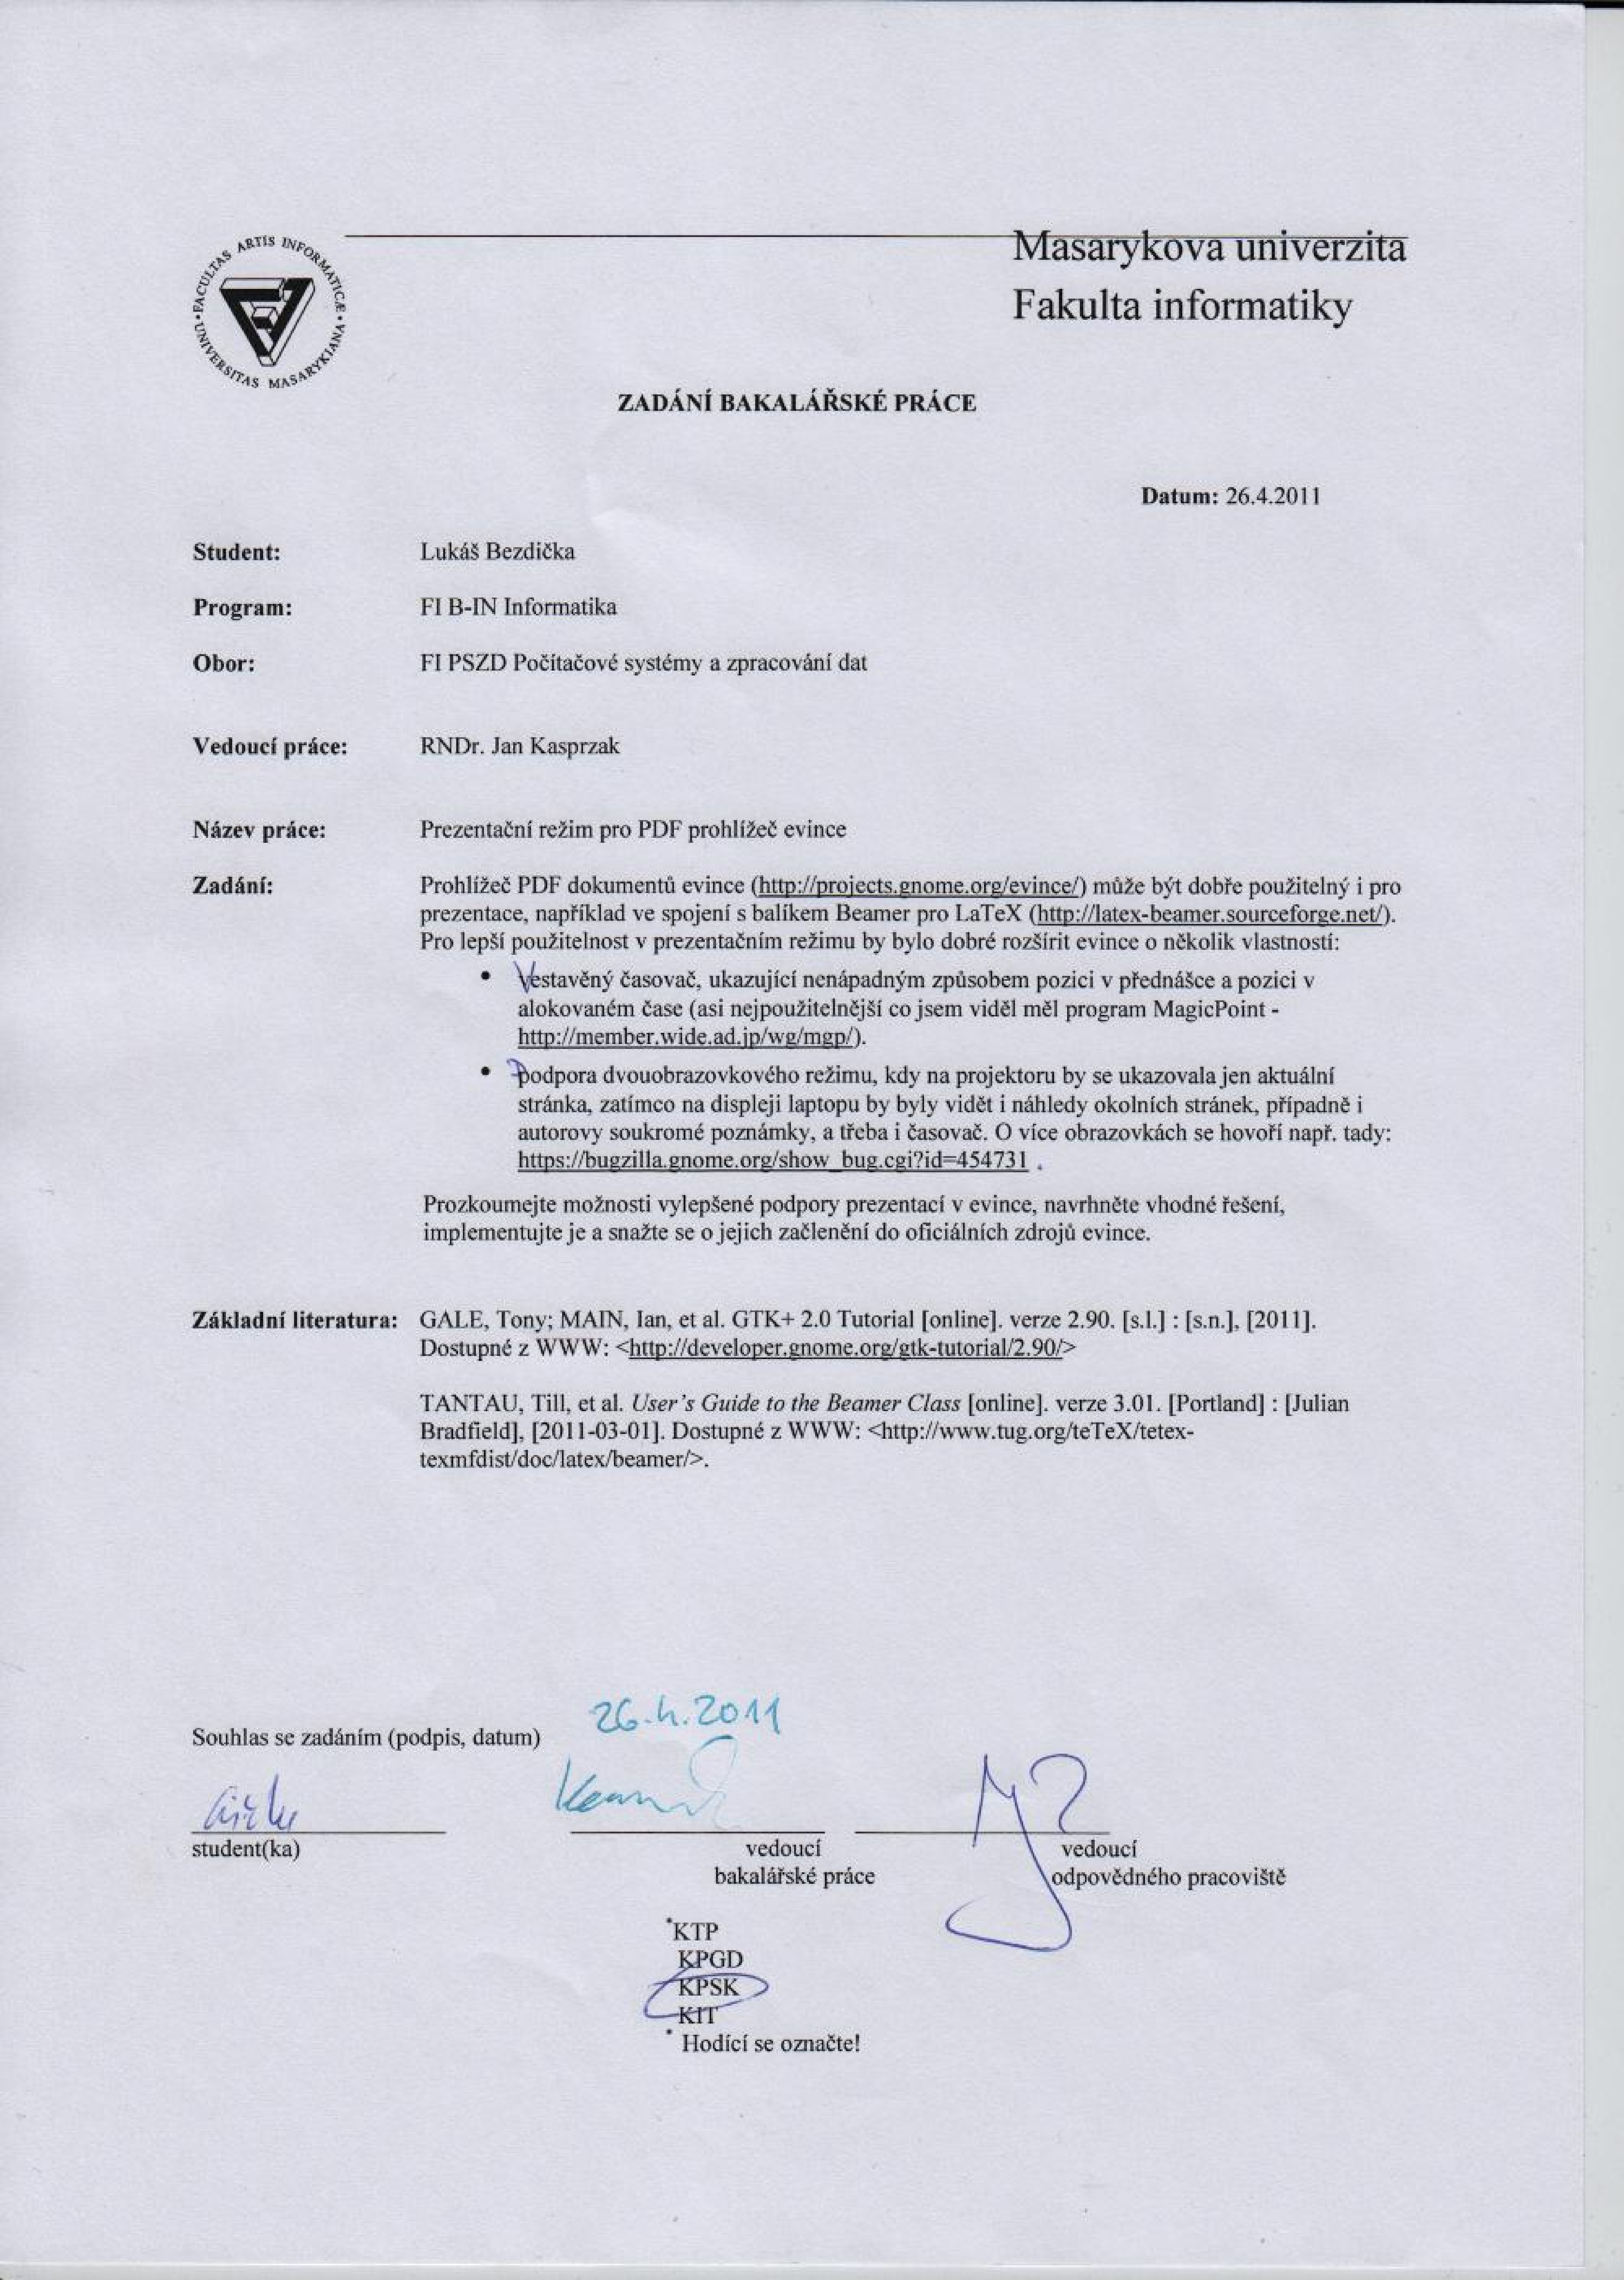
\includegraphics[bb=0 0 209 300,width=\textwidth,height=\textheight]{zadani.pdf}
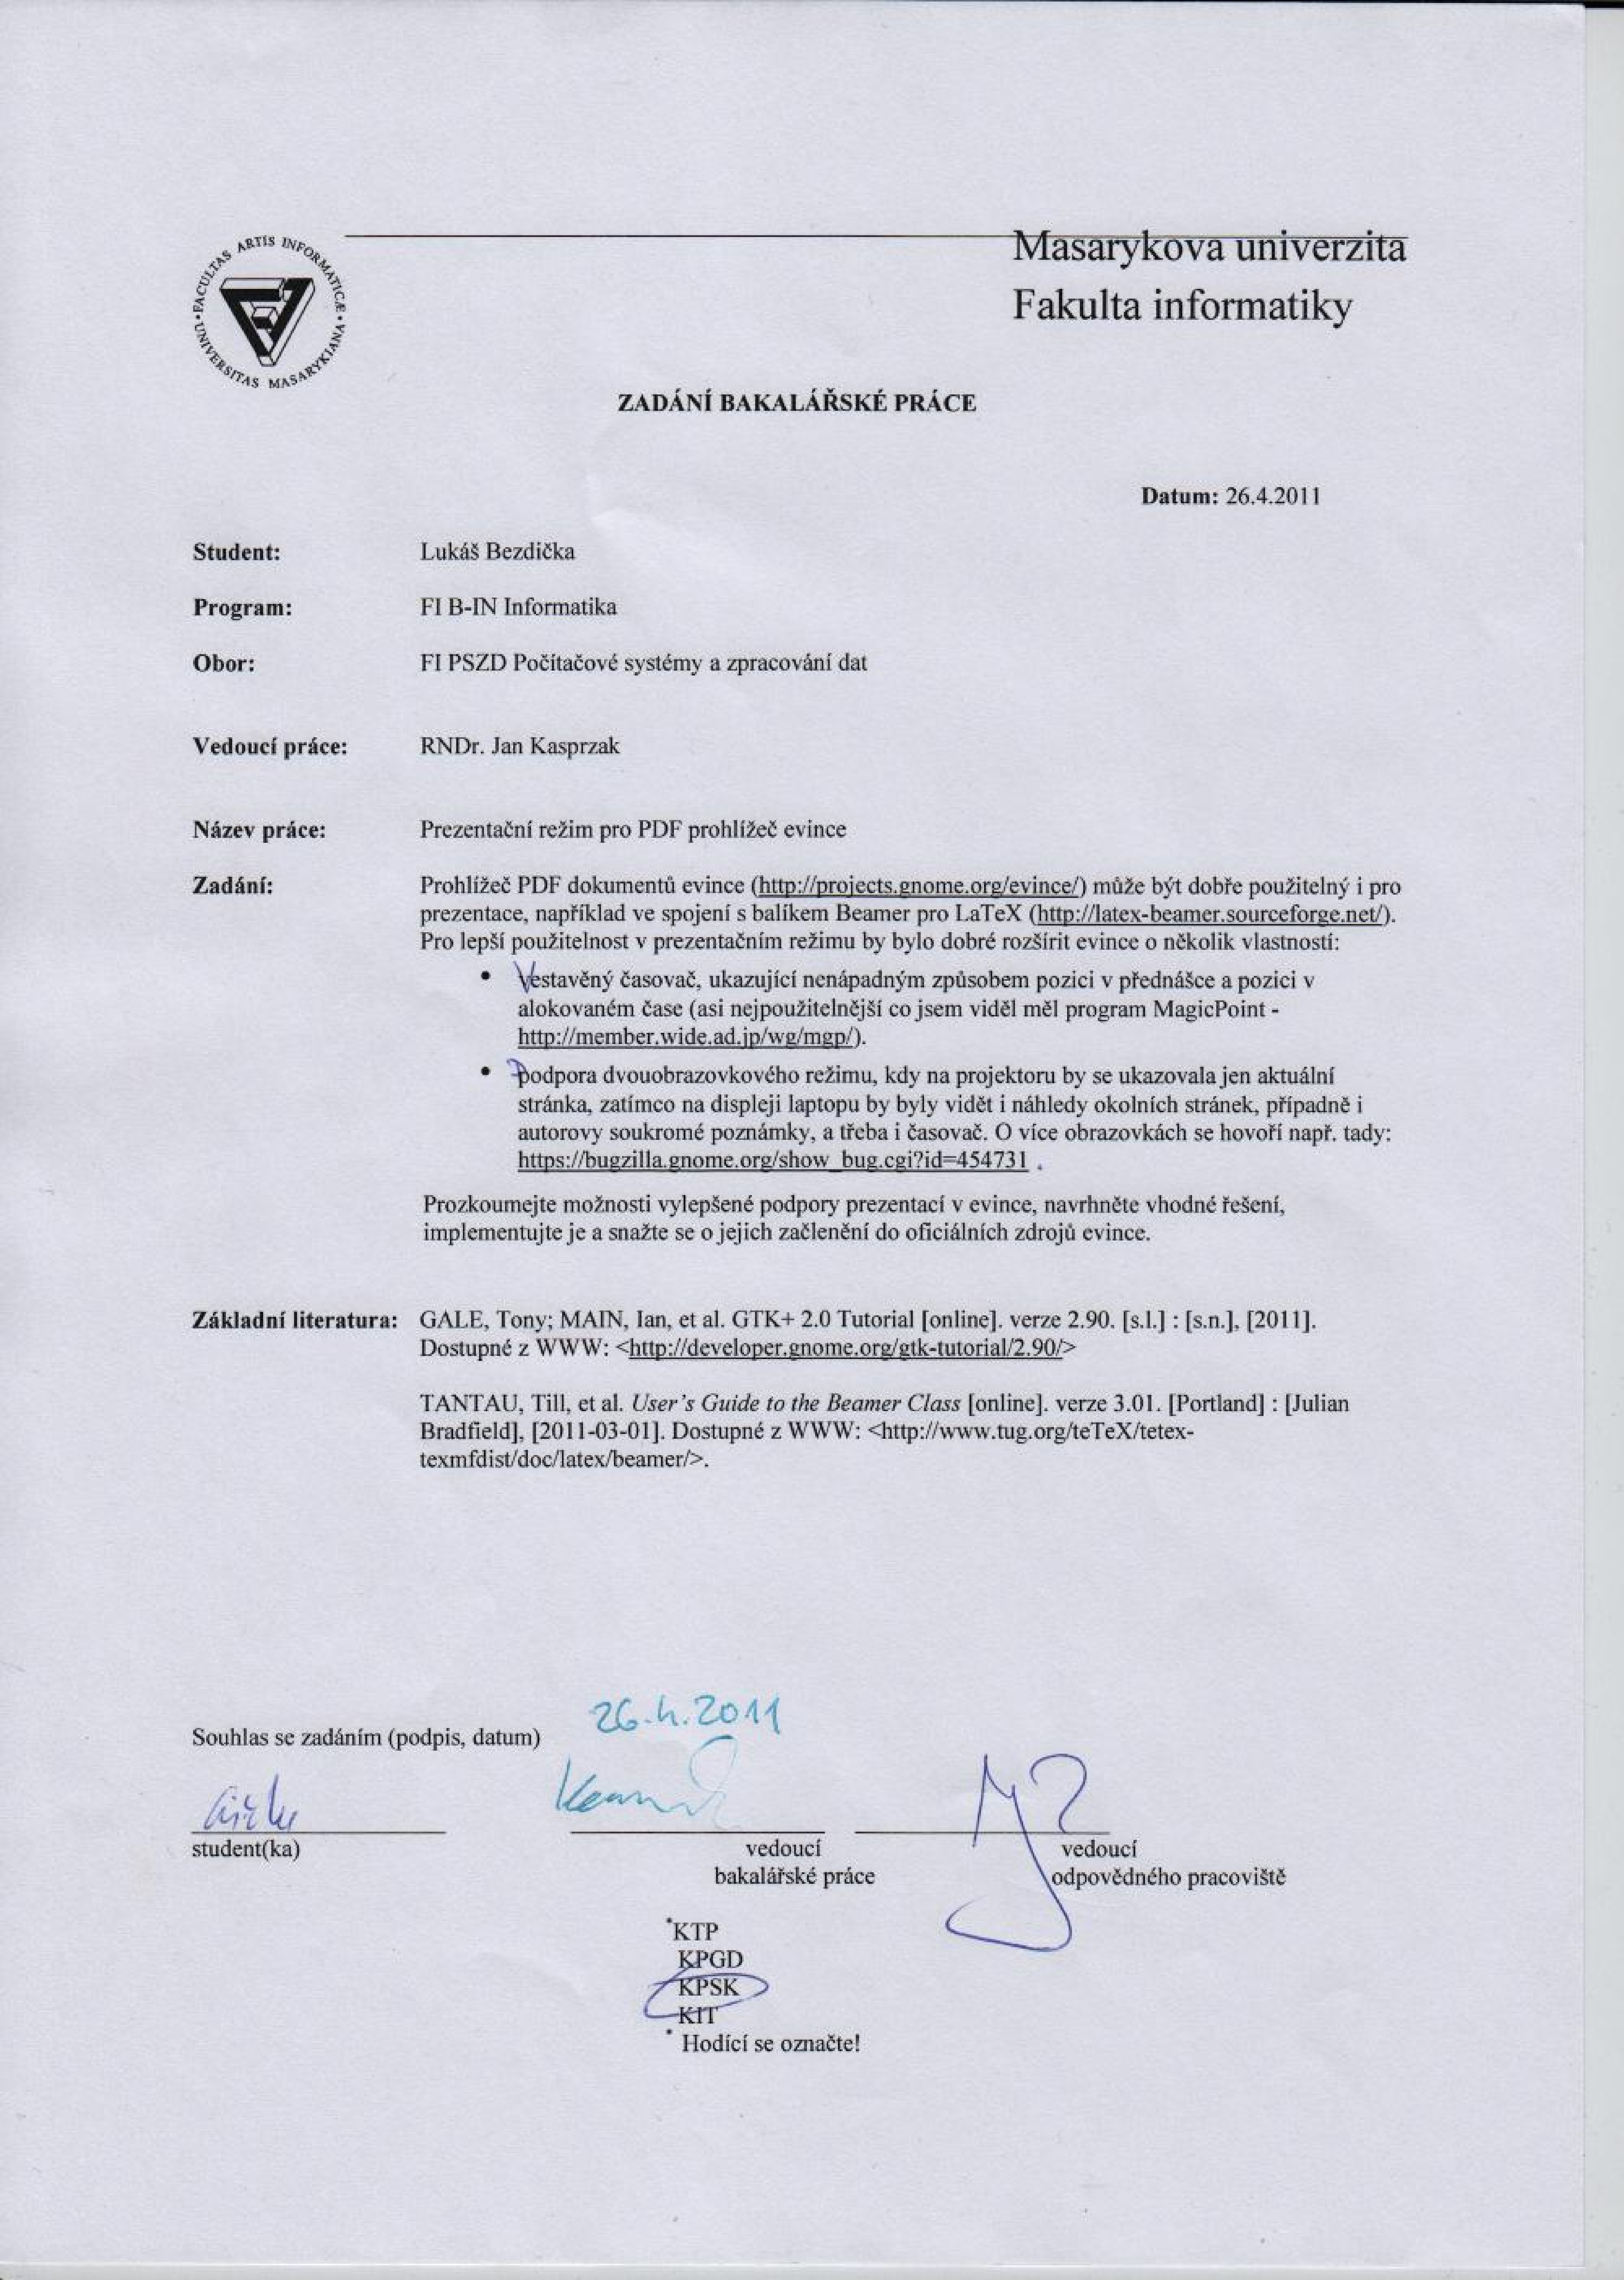
\includegraphics[height=\textheight]{zadani.pdf}
%\begin{figure}[hbtp]
%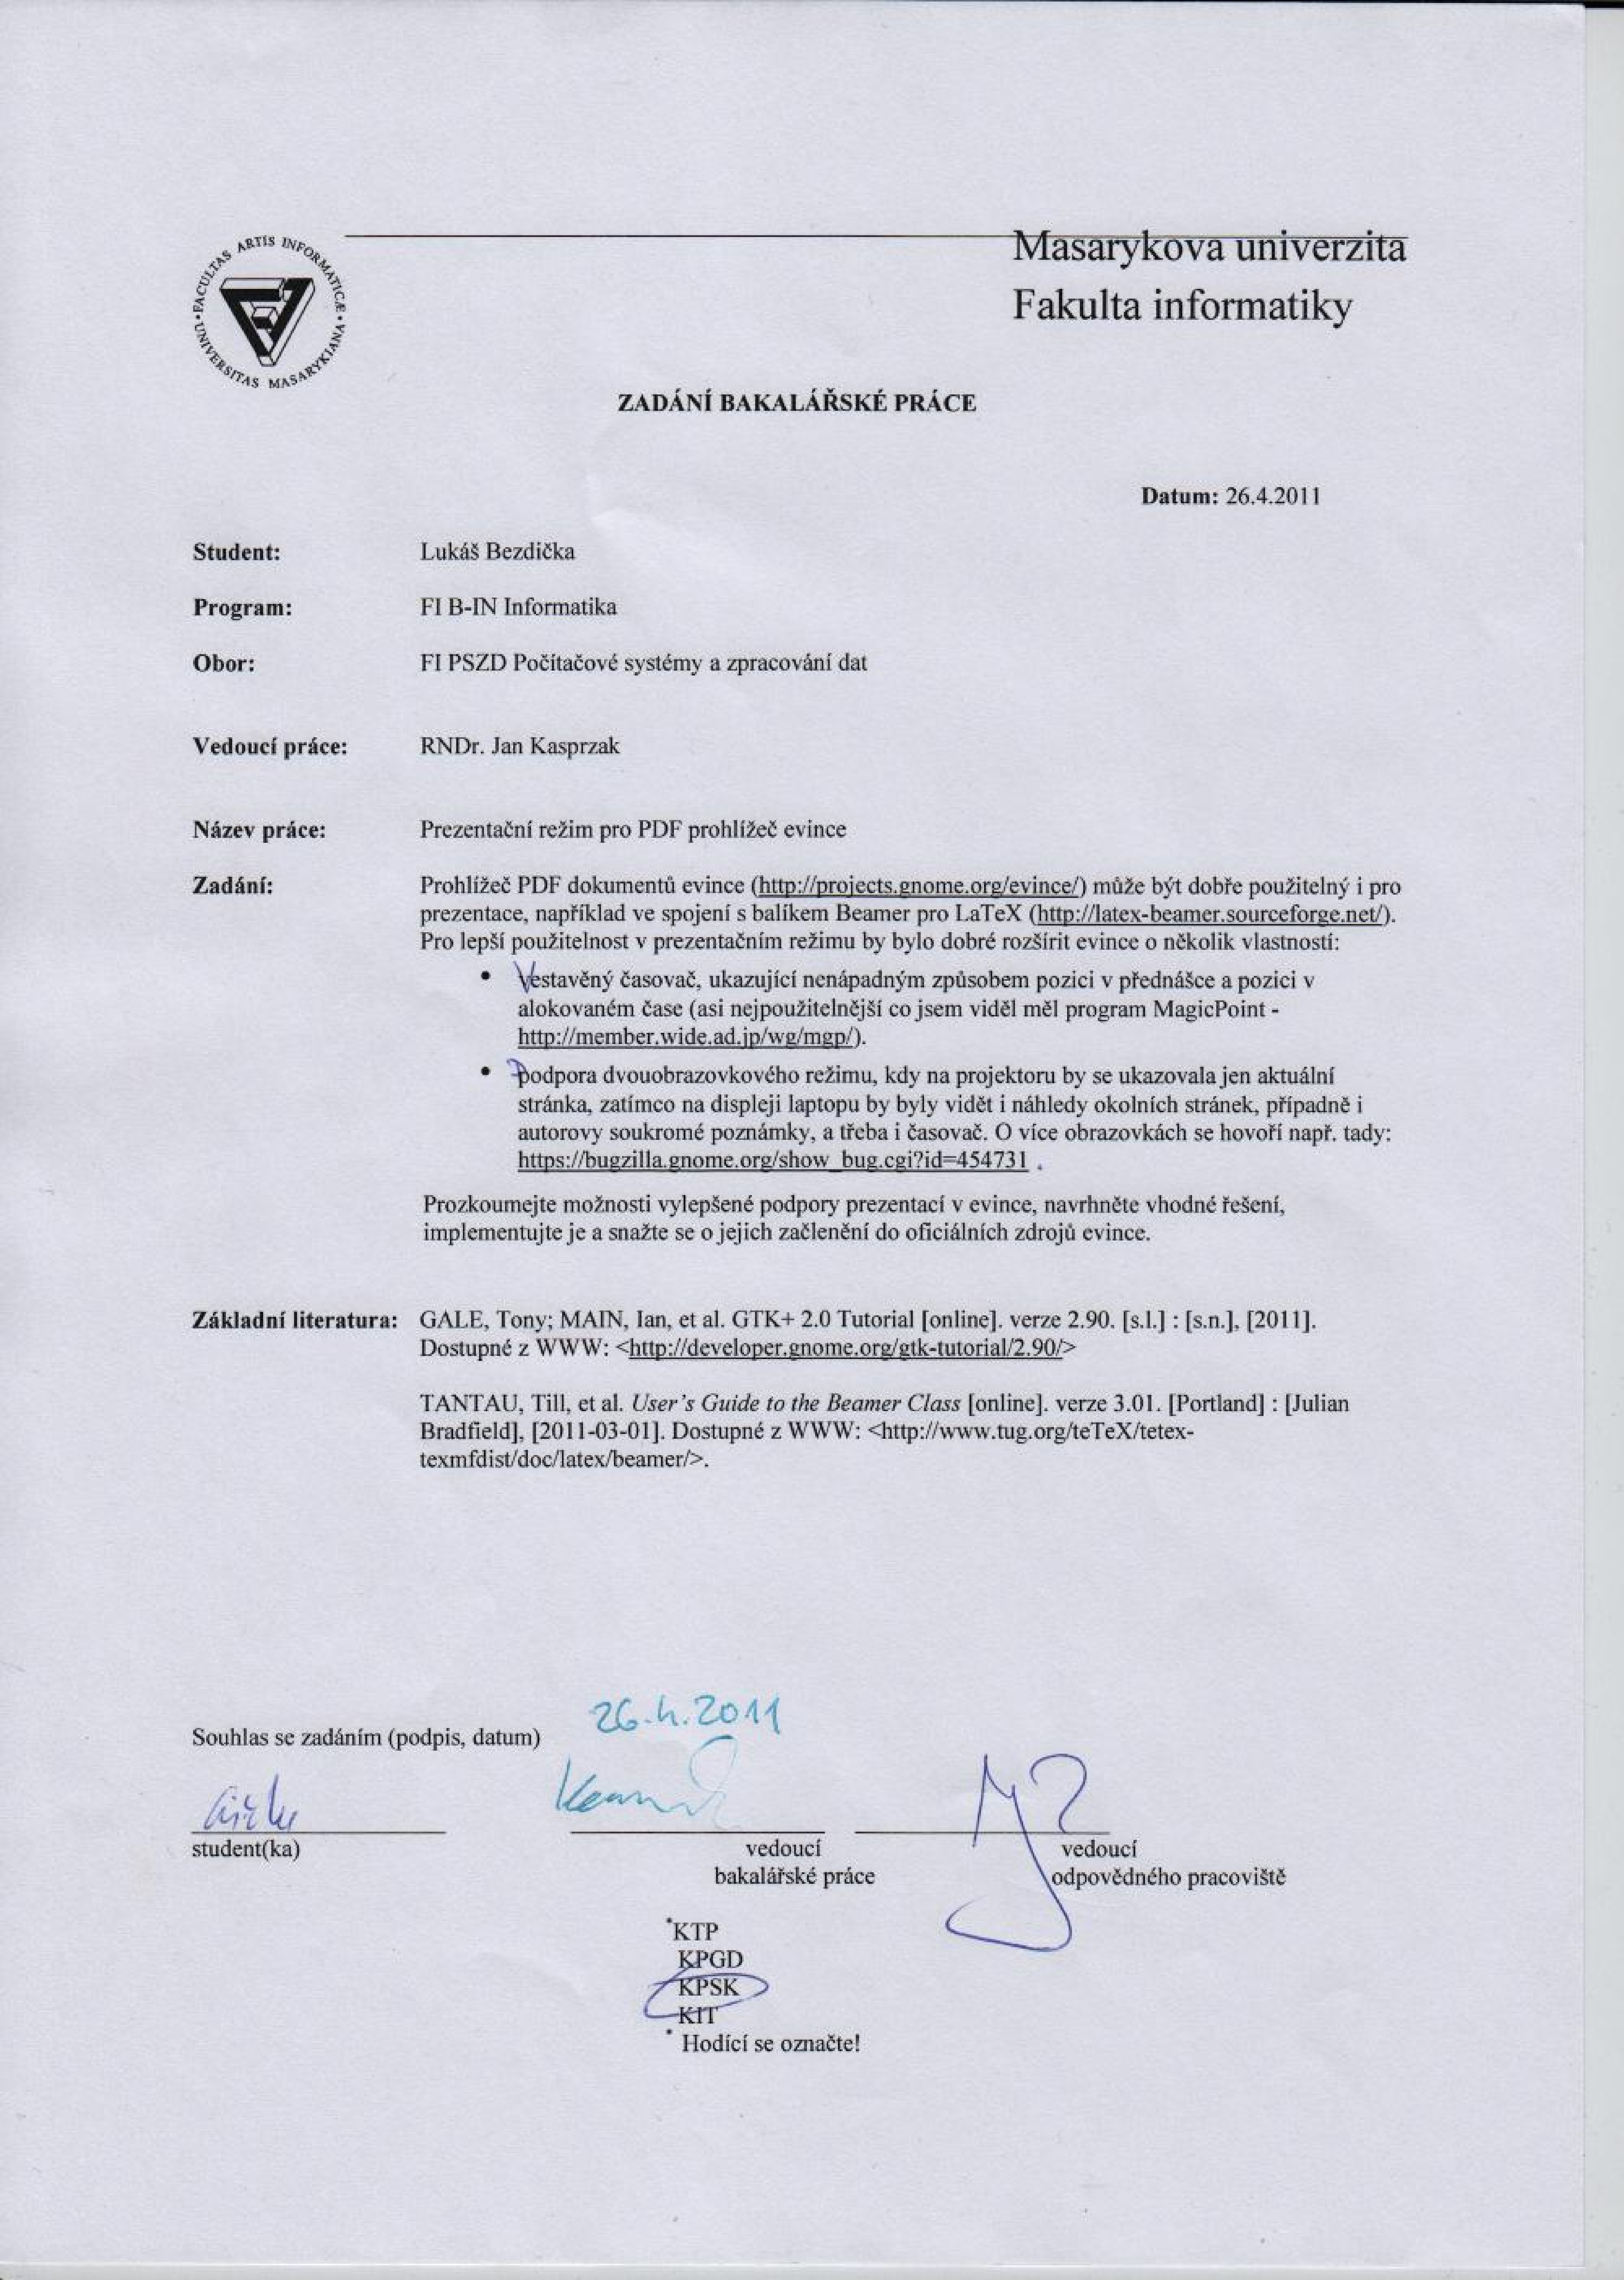
\includegraphics{zadani}
%\end{figure}


\begin{ThesisDeclaration}
\DeclarationText
\AdvisorName
\end{ThesisDeclaration}

\begin{ThesisThanks}
Rád by som poďakoval vývojárom \emph{evince} za ústretovú pomoc pri písaní práce a obzvlášť Joséovi Alisteovi. Takisto veľkou pomocou bol už existujúci kód vytvorený Johannesom Buchnerom.
\end{ThesisThanks}  

\begin{ThesisAbstract}
Prehliadač dokumentov \emph{evince} obsahuje prezentačný mód, ktorý je často používaný na prezentácie vo formáte PDF vytvorené pomocou LaTeX Beamer triedy. Táto práca pridáva podporu viacerých monitorov a pridáva grafický časovač do prezentačného módu.
\end{ThesisAbstract}

\begin{ThesisKeyWords}
Cairo, evince, GDK, GLib, GNOME, GObject, GTK+, LaTeX Beamer
\end{ThesisKeyWords}
 
\MainMatter
\sloppy
%\chapter{Predhovor}
\setcounter{tocdepth}{3}
\tableofcontents 
 
\chapter{Úvod}

Existuje nespočetné množstvo programov na tvorbu prezentácií a snáď ešte viac formátov, do ktorých je možné prezentácie uložiť. Napríklad PowerPoint a jeho formát PPT, alebo Impress a jeho formát ODP\footnote{Open Document Presentation --- otvorený formát prezentácií.}. Najtypickejší spôsob prezentácie v~dnešnej dobe je prezentácia, pri ktorej má prednášajúci svoj počítač a jeho slajdy sú premietané pripojeným projektorom na plátno za ním. Práve pre takéto prípady majú programy zabudovanú podporu pre prezentácie na viacerých monitoroch a na obrazovke počítača zobrazujú podporný materiál pre prednášajúceho. Takto sa nemusí prednášajúci publiku otáčať chrbtom. Jedným z~formátov používaných na prezentácie je aj formát PDF\footnote{Portable Document Format --- prenositeľný formát dokumentov.}. Väčšina programov na prácu s~týmto formátom ale nepodporuje viacero monitorov. Známy program používaný na formát PDF je program s~otvoreným zdrojovým kódom \emph{evince}.

\emph{Evince} obsahuje prezentačný mód, ktorý je často používaný na prezentáciu PDF dokumentov vytvorených pomocou \emph{LaTeX Beamer} triedy. Ide o~rozširujúcu triedu LaTeXu používanú miesto klasických tried dokumentu typu \texttt{article} alebo \texttt{book} \cite{abclatex}. \emph{LaTeX Beamer} trieda je navrhnutá so zreteľom na potrebu pre podporný materiál k~prezentáciám pozostávajúci zo sylabov, priesvitiek, ale aj poznámok \cite{beamer}. Tie zvyknú byť vytlačené, ale pri použití projektora môžu byť zobrazené aj na obrazovke počítača. Okrem módu poznámok je možné zobraziť na druhej obrazovke preklady alebo predošlé slajdy. O~zobrazení poznámok sa rozhoduje v~preambule dokumentu pomocou \verb|\setbeameroption{}| s~týmito nastaveniami:
\begin{description}
\item[hide notes] --- štandardné nastavenie, pri ktorom sa poznámky nepridávajú do výsledného dokumentu.
\item[show notes] --- poznámky sú zľava pripojené k~jednotlivým slajdom. Ich pozícia sa ďalej upravuje pomocou \texttt{on second \\ screen = <left,right,bottom,top>}.
\item[show only notes]  --- vytvorí samostatný dokument pozostávajúci len z~poznámok.
\end{description}

Výsledný dokument by následne mohol byť prezentovaný podobne ako prezentácie v~programoch PowerPoint alebo Impress, kde na projektore je samotná prezentácia a na obrazovke prednášajúceho sa buď zobrazujú aktuálne slajdy alebo poznámky. Alebo za pomoci \emph{XRandR} --- rozšírenia \emph{X Window} systému --- je možné spojiť viacero obrazoviek do jednej veľkej a roztiahnuť na ňu prezentáciu tak, ako to popisuje Klaus Dohmen v~článku \emph{Dual Screen Presentations with the LATEX Beamer Class under X} \cite{dohmen}. \emph{Evince} však túto funkcionalitu postráda \cite{evbug}.
\\
\\
Do úvahy prichádzali nasledujúce riešenia:
\begin{itemize}
\item Upraviť knižnicu Poppler\footnote{<\url{http://poppler.freedesktop.org/}>.} a na jej úrovni dokument rozdeliť a predať \emph{evince} dve vrstvy, ktoré by následne presunul na vybraný monitor.
\item Vyššie spomenutá možnosť spojiť obrazovky do jednej veľkej a roztiahnuť okno prezentácie tak, aby poznámky boli na jednom monitore a prezentácia na druhom. Táto možnosť by ale vyžadovala rovnaké rozlíšenie obidvoch monitorov a znemožnila by podporu viacerých platforiem.
\item Upraviť \emph{evince} na úrovni knižnice GTK+ a použiť už existujúcu triedu \texttt{EvView}. Toto riešenie sa nakoniec ukázalo ako najschodnejšie, keďže zachováva prenositeľnosť a nevyžaduje veľký zásah do už existujúceho kódu.
\end{itemize}

Bližšie informácie a popis ďalších možných riešení sa dajú nájsť v~diskusii pod hlásením o~chybe \cite{evbug}.

Cieľom bakalárskej práce v~rámci projektu \emph{evince} bolo pridať podporu pre viacero monitorov do prezentačného módu \emph{evince} v~podobe kontrolného okna na monitore prednášajúceho a časovač s~nenápadným zobrazením priebehu prezentácie.  V~prípade časovača ide o~vytvorenie ovládacieho prvku, tzv. widgetu, ktorý je následne použitý v~kontrolnom okne dvoj-obrazovkovej prezentácie. V~tomto okne prednášajúci nastaví predpokladanú dĺžku prezentácie a následne sa pri prezentácii zobrazí po úvodnom slajde na spodnej časti kontrolného okna nenápadný indikátor priebehu, podobne ako je to v~programe MagicPoint \cite{mgp}. Podpora viacerých monitorov je zameraná na prezentácie, ktoré sú vytvorené pomocou \emph{LaTeX Beamer} triedy \cite{beamer}. Ide však len o~prezentácie s~poznámkami, ktoré boli vytvorené ako samostatný súbor, pretože podpora jedného celistvého dokumentu vývojárom \emph{evince} prišla príliš špecifická pre \emph{LaTeX Beamer}, a tak by znížila šancu začlenenia výsledného kódu do projektu \emph{evince}.

Druhá kapitola popisuje platformu GNOME a jej časti. V~podkapitolách sú bližšie popísané použité časti. V~tretej kapitole je popísaný program \emph{evince} a jeho úprava. Na záver sú prezentované ďalšie možnosti rozšírenia projektu.

\chapter{GNOME Platforma}
V~roku 1997 Spencer Kimball a Peter Mattis vytvorili projekt GTK+ pre projekt GIMP\footnote{GNU Image Manipulation Program.}. V~tom istom roku Miguel de Icaza a Federico Mena založili projekt GNOME, ktorého cieľom je vytvoriť jednoduché prostredie pracovnej plochy, ktorý je postavený na GTK+. Tieto projekty zostali na seba silne naviazané a spoločne s~ďalšími tvoria platformu GNOME \ref{tab.GNOME}. Z dôvodu veľkosti platformy GNOME budú ďalej popísané len knižnice použité v~tejto práci a riešenia špecifických problémov v~rámci nich.
\begin{table}[hbtp]
\begin{center}
\begin{scriptsize}
\begin{tabular}{|c||c||c||c||c||c||c|}
\hline \multicolumn{3}{|c||}{\begin{tiny}
\textit{Užívateľské prostredie}
\end{tiny}} & \begin{tiny}
\textit{Multimédiá}
\end{tiny} & \begin{tiny}
\textit{Komunikácia}
\end{tiny} & \begin{tiny}
\textit{Ukladanie dát}
\end{tiny} & \begin{tiny}
\textit{Utility}
\end{tiny}\\
\multicolumn {1}{|c}{GTK+} & \multicolumn {1} {c} {Cairo} & \multicolumn {1} {c||} {Clutter} & GStreamer & Telepathy & EDS & Champlain \\
\multicolumn{1}{|c}{ATK} & \multicolumn{1}{c}{Pango} & \multicolumn{1}{c||}{Webkit} & Canberra & Avahi & GDA & Enchant \\ \cline{1-3}
\multicolumn{3}{|c||}{\begin{tiny}
\textit{Jadro}
\end{tiny}} & Pulseaudio &GUPnP & Tracker & Poppler \\
\multicolumn{1}{|c}{GIO} & \multicolumn{1}{c}{GLib} & \multicolumn{1}{c||}{GOBject} & & & GeoClue & \\ \hline \hline
\multicolumn{3}{|c||}{\begin{tiny}
\textit{Systémová integrácia}
\end{tiny}} & \multicolumn{4}{|c|}{{\tiny \textit{Integrácia do pracovného prostredia}}} \\
\multicolumn{1}{|c}{upower} & \multicolumn{1}{c}{udisks} & \multicolumn{1}{c||}{policykit} & \multicolumn{1}{|c}{packagekit} & \multicolumn{1}{c}{libnotify} & \multicolumn{2}{c|}{seahorse} \\
\hline 
\end{tabular}
\end{scriptsize}
\caption{Platforma GNOME \cite{GNOMEPlatform}}
\label{tab.GNOME}
\end{center}
\end{table}

\section{GLib}
Obecná knižnica funkcií GLib vznikla oddelením kódu ktorý nebol priamo špecifický pre grafické užívateľské rozhranie GTK+. GLib poskytuje abstrakciu nad platformami a používa sa ako základ programov. GLib sa dá ďalej rozdeliť na niekoľko častí. 

\textbf{GLib Fundamentals} obsahuje základné typy a ich limity, štandardné makrá, makrá na typovú konverziu a endianitu, číselné definície matematických konštánt a operácie s~desatinnou čiarkou, špeciálne makrá a podporu atomických operácií.

\textbf{GLib Core Application Support} poskytuje správu udalostí, podporu vlákien, asynchrónne fronty, dynamické moduly, správu pamäte, vstupno-výstupné kanály a systém správ.
 
\textbf{GLib Utilities}, v~ktorej sa okrem iného nachádza podpora pre časovače a funkcie na prácu s~URI\footnote{Uniform Resource Identifier --- jednotný identifikátor zdrojov definovaný v~RFC 3986 <\url{http://www.ietf.org/rfc/rfc3986.txt}>.}.

\textbf{GLib Data Types} na rozšírené dátové typy, napríklad n-árne stromy, cache a reťazce a \textbf{GLib Tools}.

\subsection{GMainLoop}
O~správu udalostí v~programoch sa stará štruktúra GMainLoop. Tieto udalosti môžu pochádzať z~rôznych zdrojov ako napríklad ukazovatele na súbory, časovače alebo vlastné zdroje pridané pomocou \texttt{g\_source}\texttt{\_attach()}. Každá udalosť má priradenú prioritu. Takisto je možné pridať funkcie, ktoré sa spustia v~prípade nečinnosti. Hlavný cyklus GMainLoop sa vytvorí pomocou funkcie \texttt{g\_main\_loop\_new()}. Po pridaní úvodných zdrojov udalostí, ktoré je možné pridávať dynamicky za behu, je potreba zavolať \texttt{g\_main\_loop\_run()}.

V~práci bolo potrebné pravidelne prekresliť časť okna. Pomocou funkcie \texttt{g\_timeout\_add\_seconds()} dôjde k~vytvoreniu zdroja udalostí a jeho pripojeniu ku kontextu hlavného cyklu. Časovač sa taktiež dá vytvoriť pomocou funkcie \texttt{g\_timeout\_add()}. Rozdiel medzi týmito funkciami je, že \texttt{\_seconds()} sa snaží zoskupiť zobudenia. Dosahuje tým väčšiu úsporu energie za cenu menšej presnosti.

\subsection{URI} 
URI je kompaktná sekvencia znakov, ktorá identifikuje abstraktný alebo fyzický zdroj. Používa sa na identifikáciu zdrojov v~sieti Internet. URI je spojením URL\footnote{Uniform Resource Locator --- jednotný lokátor zdrojov definovaný v~RFC 1738 <\url{http://www.ietf.org/rfc/rfc1738.txt}>} na určenie lokácie zdroja a URN\footnote{Uniform Resource Name --- jednotný názov zdrojov definovaný v~RFC 1737 <\url{http://www.ietf.org/rfc/rfc1737.txt}>} na identifikáciu zdroja. Na obrázku \ref{obr.URI} zobrazená syntax URI je definovaná takto:
\begin{description}
\item[schéma] používa sa na špecifikáciu protokolu a obmedzenie syntaxe URI identifikátorov. Schémy by mali byť registrované IANA\footnote{Internet Assigned Numbers Authority <\url{http://www.iana.org/}>}.
\item[hierarchická časť] delí sa na dve časti, a to špecifikáciu autority (začína s~\uv{//}), ktorá môže obsahovať informácie o~užívateľovi a cestu ku zdroju.
\item[dotaz] nepovinná nehierarchická časť identifikátora obsahujúca dodatočné identifikačné informácie. Od cesty sa oddeľuje otáznikom.%ref wiki
\item[fragment] nepovinná časť oddelená znakom \uv{\#} na nepriamu identifikáciu sekundárneho zdroja na základe primárneho zdroja a doplňujúcej informácie. Môže ísť o~nejakú konkrétnu časť zdroja alebo o~iný zdroj definovaný týmito reprezentáciami.
\end{description}
Na prevod medzi názvom súboru a URI poskytuje GLib makrá \texttt{g\_filename\_from\_uri()} a \texttt{g\_filename\_to\_uri()}.

\begin{figure}[hb]
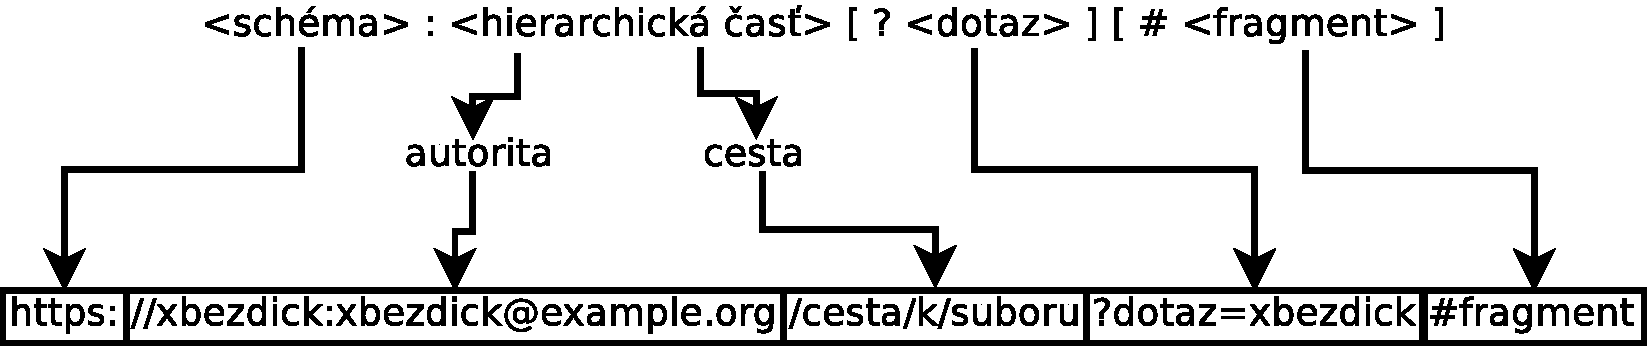
\includegraphics[width=\linewidth]{Diagram1.pdf}
\caption{Schéma URI s~príkladom.}
\label{obr.URI}
\end{figure}

\section{GObject}
GLib Object System je objektovo orientovaný framework pre jazyk C postavený na GLib. GObject je navrhnutý tak, aby bolo možné exportovať jeho C-API\footnote{API --- rozhranie pre programovanie aplikácií.} do ostatných jazykov za pomoci, tzv. lepiaceho kódu\footnote{<\url{http://developer.gnome.org/gobject/stable/ch01s02.html}>}.

Súčasťou GLib je dynamický typový systém postavený na štruktúre GType\footnote{<\url{http://developer.gnome.org/gobject/unstable/chapter-gtype.html}>}. Táto štruktúra v~skratke definuje veľkosť triedy, inicializačné a deštrukčné funkcie, veľkosť inštancie triedy, pravidlá inštancií\footnote{V C++ typ nového operátora.}, kopírovacie funkcie atď.

Knižnica GObject poskytuje základnú objektovú triedu GObject\footnote{<\url{http://developer.gnome.org/gobject/unstable/}>}. GObject neumožňuje viacnásobnú dedičnosť a je implementovaný na spôsob Javových rozhraní. Každá GObject trieda sa implementuje pomocou minimálne dvoch štruktúr, ale zvykom je použiť aspoň tri --- štruktúru triedy, štruktúru inštancií a privátnu štruktúru inštancií --- keďže jazyk C nemá prístupové modifikátory \texttt{public}, \texttt{protected} alebo \texttt{private}. GObject definuje určitú formu kódu, tzv. boilerplate\footnote{<\url{http://developer.gnome.org/gobject/stable/howto-gobject.html}>}.
Pre hlavičkové súbory je boilerplate popísaný na obrázku \ref{ev-presentation-timer.h}.
\begin{figure}[hbpt]
\begin{tiny}
\begin{verbatim}
/*
 *Copyright a licenčné informácie
 */
/*Kontrola inklúzie.*/
 #ifndef _EV_PRESENTATION_TIMER_H_
 #define _EV_PRESENTATION_TIMER_H_
/*Špeciálne makro, ktoré v~prípade c++ kompilátora pridá extern okolo hlavičky.*/
 G_BEGIN_DECLS
 typedef struct _EvPresentationTimerClass        EvPresentationTimerClass;
 typedef struct _EvPresentationTimer             EvPresentationTimer;
 typedef struct _EvPresentationTimerPrivate      EvPresentationTimerPrivate;
/* Typové makrá */
 #define EV_TYPE_PRESENTATION_TIMER              (ev_presentation_timer_get_type ())
 #define EV_PRESENTATION_TIMER(object)           (G_TYPE_CHECK_INSTANCE_CAST ((object), EV_TYPE_PRESENTATION_TIMER, \
                                                  EvPresentationTimer))
 #define EV_PRESENTATION_TIMER_CLASS(klass)      (G_TYPE_CHECK_CLASS_CAST ((klass), EV_TYPE_PRESENTATION_TIMER, \
                                                  EvPresentationTimerClass))
 #define EV_IS_PRESENTATION_TIMER(object)        (G_TYPE_CHECK_INSTANCE_TYPE ((object), EV_TYPE_PRESENTATION_TIMER))
 #define EV_IS_PRESENTATION_TIMER_CLASS(klass)   (G_TYPE_CHECK_CLASS_TYPE ((klass), EV_TYPE_PRESENTATION_TIMER))
 #define EV_PRESENTATION_TIMER_GET_CLASS(object) (G_TYPE_INSTANCE_GET_CLASS ((object), EV_TYPE_PRESENTATION_TIMER, \
                                                  EvPresentationTimerClass))
 struct _EvPresentationTimerClass
 {
         GtkDrawingAreaClass parent_class;
         /* členovia triedy */
 };
 struct _EvPresentationTimer 
 {
         GtkDrawingArea                  parent_instance;
         /*privátna štruktúra je potom definovaná v~.c súbore*/
         EvPresentationTimerPrivate     *priv;
         /*členovia inštancie*/ 
};
 void                    ev_presentation_timer_set_pages         (EvPresentationTimer *ev_timer,
                                                                  guint pages);
 void                    ev_presentation_timer_set_page          (EvPresentationTimer *ev_timer,
                                                                  guint page);
 void                    ev_presentation_timer_start             (EvPresentationTimer *ev_timer);
 void                    ev_presentation_timer_stop              (EvPresentationTimer *ev_timer);
 void                    ev_presentation_timer_set_time          (EvPresentationTimer *ev_timer,
                                                                  gint time);
 GType                   ev_presentation_timer_get_type          (void);
 GtkWidget              *ev_presentation_timer_new               (void);
 
 G_END_DECLS
 #endif
\end{verbatim}
\end{tiny}
\caption{Okomentovaná ukážka kódu.}
\label{ev-presentation-timer.h}
\end{figure}

Pri inicializácii triedy \texttt{ev\_presentation\_timer\_class\_init()} musí funkcia \texttt{g\_type\_class\_add\_private()} registrovať privátnu štruktúru pre triedu\cite{gprivate}. Pri alokácii objektu sú privátne štruktúry pre typy a typy ich rodičov sprístupnené sekvenčne v~rovnakom pamäťovom bloku ako ich verejné štruktúry. Nakoniec pri inicializácii inštancie v~tomto prípade \texttt{ev\_presentation\_timer\_init()} sa za pomoci makra \texttt{G\_TYPE\_INSTANCE\_GET\_PRIVATE()} získa ukazovateľ na privátnu dátovú štruktúru. Na implementáciu \texttt{ev\_presentation\_timer\_get\_type()} funkcie a na definíciu ukazovateľa na rodičovskú triedu sa používa makro \texttt{G\_DEFINE\_TYPE}.

GObject poskytuje štandardný get/set mechanizmus pre objektové vlastnosti. Vlastnosti sa registrujú pri inicializácii objektu volaním funkcie \texttt{g\_object\_class\_install\_property()}.

Pri riešení problému bolo potrebné pridať vlastnosť \texttt{PROP\_PAGE} do \texttt{EvViewPresentation}. \texttt{PROP\_PAGE} odkazuje na číslo aktuálnej stránky. Jej obsah sa získa pomocou \texttt{g\_object\_get\_property()} a nastavuje sa pomocou \texttt{g\_object\_set\_property()}. Túto funkčnost zabezpečuje prepísanie štandardných funkcií GObject triedy počas inicializácie triedy vo funkcii \texttt{ev\_view\_presentation\_class\_init()}. Následne pri zmene vlastnosti môže objekt vyslať \uv{nofity} signál pre danú vlastnosť pomocou funkcie \texttt{g\_object\_notify()}.

Systém správ GObjectu sa skladá zo signálov a uzáverov\footnote{<\url{{http://developer.gnome.org/gobject/unstable/chapter-signal.html\#closure}}>}. Uzávere sú kľúčový koncept pre asynchrónne doručovanie signálov široko používaný v~GNOME. Uzávere sú abstrakciou generického spätného volania pre signály. Štruktúra uzáveru obsahuje tri objekty:
\begin{itemize}
\item ukazovateľ na vyhradenú funkciu, tzv. callback.
\item ukazovateľ na užívateľské dáta ktorý je predaný callbacku pri volaní uzáveru.
\item ukazovateľ na funkciu deštruktora uzáveru.
\end{itemize}
Princíp uzáver funguje tak, že program spí v~hlavnom cykle pokiaľ sa neudeje nejaká udalosť a kontrola je následne predaná vyhradenej funkcii. Udalosť je reprezentovaná odoslaným signálom z~objektu, v~ktorom sa táto udalosť udiala. Na jednotlivé signály sa pripája manipulátor (uzávera alebo \uv{handler}), ktorý tieto signály odchytí a zavolá vyhradenú funkciu. Zjednodušená verzia pripojenia signálov prebieha pomocou volania:
\begin{verbatim}
gulong g_signal_connect( gpointer      *objekt,
                         const gchar   *nazov,
                         GCallback     funkcia,
                         gpointer      uziv_data );
\end{verbatim} Pre ktoré bude vyhradená funkcia vyzerať približne takto: 
\begin{verbatim}
void callback_func( GtkWidget *objekt,
                    gpointer   uziv_data );
\end{verbatim}
A~pokiaľ chceme predať callback funkcii len jeden objekt je treba použiť \texttt{g\_signal\_connect\_swapped()}.

\section{GTK+}
GIMP Toolkit je sada knižníc určená na tvorbu rozhrania grafických aplikácií, tzv. widgetov. Okrem programovacieho jazyka C knižnica podporuje mnoho ďalších za pomoci jazykových väzieb. GTK+ používa tieto knižnice:
\begin{description}
\item[GLib] používa napríklad obalením hlavného cyklu do \texttt{gtk\_main()}.
\item[GObject] každý widget je potomkom objektu GObject.
\item[GIO] VFS\footnote{Virtual File System - systém na abstrakciu nad súborovými systémami} API na abstrakciu vstupno-výstupných operácií.
\item[cairo] na vykresľovanie widgetov.
\item[Pango] na prácu s~textom.
\item[ATK] toolkit na zvýšenie dostupnosti pre zrakovo, či sluchovo postihnutých ľudí.
\item[GdkPixBuf] malá knižnica na tvorbu objektov z~obrázkov.
\item[GDK] poskytujúca abstrakčnú vrstvu nad okennými systémami ako napríklad X11, Winows \dots
\end{description}
Spojením týchto knižníc dodáva GTK+ flexibilitu a zjednodušuje prenositeľnosť na iné platformy.
Programy postavené na GTK+ inicializujú GTK+ volaním funkcie \texttt{gtk\_init()}. Táto funkcia nastaví napríklad štandardný handler pre signály, mapu farieb atď. Následne je nutné vytvoriť základné widgety a volaním \texttt{gtk\_main()} skočiť do hlavného cyklu. Triedy GTK+ sú usporiadané hierarchicky\footnote{<\url{http://developer.gnome.org/gtk/unstable/ch01.html}>} a na základe tejto hierarchie je pri tvorbe nového widgetu dobré správne zvoliť rodičovskú triedu tak, aby implementovala čo najviac funkcionality a aby ďalšie rozšírenia pozostávali z~nových funkcií alebo len prepísania štandardných funkcií triedy.
\subsection{GtkWidget}
GtkWidget je abstraktnou základnou triedou pre všetky widgety\footnote{<\url{http://developer.gnome.org/gtk/unstable/GtkWidget.html}>}, či už ide o~okno, tlačidlo alebo kontajner. Táto trieda sa stará o~životný cyklus, stavy a štýly widgetov. Životný cyklus widgetu pozostáva z~vytvorenia nového objektu, pripojenia handlerov a signálov --- inicializácii (\texttt{realize}) --- presunutia widgetu na jeho pozíciu a určenie veľkosti (\texttt{size-request, size-allocate, configure-event}), zobrazenia widgetu (\texttt{show}) a následného vykreslenia (\texttt{draw}), ukončenia (\texttt{delete-event}) a mnoho ďalších. Napríklad prepisom funkcie \texttt{draw} počas inicializácie triedy a vytvorením vlastnej \texttt{\_draw()} funkcie sa dostaneme ku cairo kontextu widgetu a je možné ovládať vykreslenie widgetu.
\subsection{GtkWindow}
Trieda GtkWindow popisuje okno a jeho vlastnosti, ktoré, ako potomok triedy \texttt{GtkContainer}, môže obsahovať ďalšie widgety. Pomocou tejto triedy je možné narábať podobne ako s~oknom narába užívateľ. Funkcia \texttt{gtk\_window\_move()} slúži na presunutie okna na danú pozíciu. Túto operáciu má vykonať správca okien, ten ju však bude ignorovať, dokým okno nieje naozaj zobrazené. V~práci bolo nutné čé najskôr presunúť kontrolné okno a okno s~prezentáciou na svoje pozície. Na to však museli prebehnúť všetky udalosti a okno sa muselo zobraziť. Preto bolo nutné prejsť niekoľkými iteráciami hlavného cyklu ako je zobrazené v~nasledujúcej ukážke kódu \ref{iterate}.
\begin{figure}[hbtp]
\begin{tiny}
\begin{verbatim}
	/* Wait for windows to get shown before moving them */
	while(gtk_events_pending())
		gtk_main_iteration();
	/* something like http://mail.gnome.org/archives/gtk-list/2008-June/msg00061.html */
\end{verbatim}
\end{tiny}
\caption{Kód na dobehnutie čakajúcich udalostí pomocou iterácie hlavného cyklu.}
\label{iterate}
\end{figure}
%TODO FINISH ME
%\subsection{packing widgets}
\section{Cairo}
Cairo je knižnica určená na kreslenie 2D vektorov napísaná v~jazyku C a rovnako ako GTK+ je použiteľná v~ostatných programovacích jazykoch za pomoci jazykových väzieb. Pomocou caira je možné kresliť do viacerých výstupov ako napríklad PDF, PNG\footnote{Portable Network Graphics.}, GtkWindow. Model kreslenia pomocou knižnice cairo pozostáva z~týchto definícií:
\begin{description}
\item[Context] reprezentuje kontext v~ktorom chceme kresliť. To znamená, že popisuje čo, kam a ako.
\item[Surface] reprezentuje povrch na ktorý chceme kresliť. Môže to byť ktorýkoľvek z~typov definovaných v~\texttt{\_cairo\_surface\_type}.
\item[Path] reprezentuje cestu. Pri analógii s~maľovaním reprezentuje ťah štetca.
\item[Source] reprezentuje zdroj pozostávajúci z~farby, gradientu, obrázku alebo vzoru. V~podobnej analógii ako v~predošlom prípade reprezentuje farbu štetca.
\item[Mask] reprezentuje šablónu, podľa ktorej sa aplikuje kresba.
\end{description}
Kreslenie pomocou cairo prebieha tak, že sa vytvorí kontext \texttt{cairo\_t}, nastaví sa mu povrch a nastavenia. V~prípade tejto práce išlo o~kontext s~povrchom widgetu, ktorý bol špeciálne z~tohto dôvodu potomkom triedy \texttt{GtkDrawingArea}. Následne pomocou funkcie \texttt{cairo\_set\_source\_rgb()} sa vyberie farba, za pomoci \texttt{cairo\_set\_line\_width()} určí šírka čiary, \texttt{cairo\_move\_to()} presunie na východziu pozíciu, \texttt{cairo\_line\_to()} určí vlastnosti cestu a funkcia \texttt{cairo\_stroke()} následne nakreslí čiaru podľa zvolenej cesty a šírky. Cairo ponúka mnoho ďalších funkcií --- napríklad kreslenie obdĺžnikov \texttt{cairo\_rectangle()}, vyplnenie cesty \texttt{cairo\_fill()} --- bližšie popísaných v~dokumentácii projektu\cite{cairodoc}.
\chapter{Evince}
Prehliadač dokumentov \emph{evince} podporuje formáty PDF, PS\footnote{Post Script.}, DjVu\footnote{Formát na ukladanie naskenovaných dokumentov.}, TIFF\footnote{Tag Image File Format.} a DVI\footnote{DeVice Independent.}. Bol vytvorený ako prepis programu GPdf\footnote{<\url{http://freshmeat.net/projects/gpdf/}>.}, ktorý vznikol z~Xpdf\footnote{<\url{http://foolabs.com/xpdf/about.html}>.}, s~cieľom nahradiť viaceré prehliadače dokumentov v~GNOME jednou jednoduchou aplikáciou \cite{evince}. \emph{Evince} z~projektu Xpdf používa knižnicu Poppler a takisto ako GPdf je založený na knižnici GTK+. Program \emph{evince} je štruktorovaný do:
\section{backend}
V~backende sa nachádzajú knižnice fungujúce ako prípojné body pre knižnice na prácu s~jednotlivými formátmi. Napríklad knižnica \texttt{libpdfdocument} slúži na pripojenie knižnice Poppler, ktorá sa už stará o načítanie a vykreslenie PDF dokumentu. Na pridanie podpory nového formátu do \emph{evince} teda stačí mať knižnicu, ktorá tento formát vie vykresliť na povrch caira a vytvoriť knižnicu v backende implementujúcu rozhranie \texttt{libdocument}.
\section{libdocument}
Knižnica libdocument obsahuje triedu \texttt{EvDocument} slúžiacu na zjednotenie operácií s dokumentami. Definuje rozhranie pre knižnice na prácu s jednotlivými formátmi a slúži na načítanie dokumentu z URI.
\section{libview}
Ide o knižnicu na prácu s náhľadmi na dokument starajúcu sa o zobrazenie dokumentu. Obsahuje triedy \texttt{EvDocumentModel} a \texttt{EvView} zjednocujúce prácu s náhľadmi ale aj triedu \texttt{EvViewPresentation} reprezentujúcu prezentačný mód \emph{evince}. Cieľom libview je umožniť vývojárom iných aplikácií zabudovať \texttt{EvView} widget do ich programov a mať tak vstavaný prehliadač dokumentov bez nutnosti použiť užívateľské rozhranie \emph{evince}.
\section{shell}
Tvorí jadro programu \emph{evince}, obsahuje väčšinu stavebných widgetov programu. V jadre je definovaná trieda okna programu \texttt{EvWindow}, bočný panel \texttt{EvSidebar}, metadáta \texttt{EvMetadata} a ďalšie triedy.
\subsection{metadata}
Program evince plne využíva celý rozsah platformy GNOME, jednou z jej ešte nepopísaných častí v tejto práci je GIO. Ide o knižnicu pre vstupno-výstupné operácie GVFS --- virtuálneho súborového systému GNOME --- poskytujúcu aj možnosť ukladať si metadáta. Ide o dáta o dátach používané programami na uloženie špecifických nastavení pre jednotlivé súbory \cite{metad}. Napríklad program evince si takto ukladá informácie o veľkosti okna, aktuálnej strane atď. viac v ukážke \ref{meta}.
\begin{figure}[hbpt]
\begin{tiny}
\begin{verbatim}
$ gvfs-info -a "metadata::*" gtk-tut.pdf 
attributes:
  metadata::evince::page: 2
  metadata::evince::sidebar_size: 170
  metadata::evince::sidebar_visibility: 1
  metadata::evince::window_height: 751
  metadata::evince::window_maximized: 1
  metadata::evince::window_width: 1280
  metadata::evince::window_x: 0
  metadata::evince::window_y: 49
\end{verbatim}
\end{tiny}
\caption{Metadáta o súbore \texttt{gtk-tut.pdf} vypísané pomocou \texttt{gtk-info}.}
\label{meta}
\end{figure}


\texttt{EvMetadata} obsahuje get/set funkcie na prácu s metadátami a ukladá ich vo formáte \texttt{metadata::evince::key}. Pomocou metadát je v práci vyriešené zapamätanie si času potrebného na prezentáciu, umiestnenie okien a URI súbora s poznámkami.

\chapter{Úprava programu \emph{evince}}
Práca pozostávala z~vytvorenia \texttt{EvDSCWindow} triedy (potomoka \texttt{GtkWindow}), pomocou ktorej je vytvorené kontrolné okno v~\texttt{EvWindow} vo funkci \texttt{ev\_window\_run\_presentation()}. Do funkcie \texttt{ev\_window\_run\_presentation()} bola pridaná kontrola dispozície dvoch alebo viacerých monitorov. Kontrolné okno pozostáva z náhľadu na dokument, bočného panelu, tzv. sidebar, rozširujúceho panelu obsahujúceho nasledujúce tlačidlá: prepínanie monitorov, otvorenie súboru s poznámkami, ukončenie prezentácie, zobrazenie sidebaru a nastavenie časovača. Ďalej sa v kontrolnom okne nachádza časovač \texttt{EvPresentationTimer}. Po vytvorení kontrolného okna je mu nutné predať ukazovatele na pôvodné okno, aktuálny dokument, pohľad prezentácie a metadáta pomocou funkcie \texttt{ev\_dscwindow\_set\_presentation()}. \texttt{EvDSCWindow} následne nastaví \texttt{EvDocumentModel} náhľadu na poznámky a sidebaru, pripojí signály \texttt{destroy} a \texttt{notify::page} pre pohľad prezentácie a \texttt{notify::page} pre \texttt{EvDocumentModel} na callbacky. \texttt{Destroy} signál je napojený na funkciu GTK+ \texttt{gtk\_widget\_destroy()}. Signály \texttt{notify::page} slúžia na synchronizovanie strán medzi jednotlivými náhľadmi. Callbacky pre tieto signály následne volajú funkciu \texttt{ev\_dscwindow\_set\_page()}, ktorá nastaví správnu stranu na všetkých náhľadoch a časovači, ak išlo o presun z úvodného slajdu, spustí časovač.
\section{Prepínanie monitorov}
O prepínanie monitorov sa starajú funkcie \texttt{ev\_dscwindow\_switch\_monitors()} na zámenu monitorov a \texttt{ev\_dscwindow\_windows\_placement()} na následné presunutie okien. %GDK TODO
\section{Poznámky}
Po stlačení tlačidla na načítanie poznámok sa emituje signál \texttt{clicked}, na ktorý je pripojený callback \texttt{ev\_dscwindow\_notes\_interaction()}. V tejto funkcii sa vytvorí \texttt{GtkFileChooserDialog} widget určený na vytvorenie dialógového okna na vyberanie súborov a v prípade existencie metadát je mu predaná URI k naposledy použitým poznámkam aktuálneho dokumentu. Po spustení dialógu pomocou funkcie \texttt{gtk\_dialog\_run()} a prijmutí \texttt{GTK\_RESPONSE\_ACCEPT} je dokument načítaný do \texttt{EvDocument} a vytvorí sa \texttt{EvDocumentModel}, ktorý je potom predaný náhľadu na poznámky pomocou funkcie \texttt{ev\_view\_set\_model} a je pripojený callback na jeho \texttt{notify::page} signál.
\section{Inicializácia a ukončenie}
Inicializácia a ukončenie je definovaná tým, že každý widget je potomok \texttt{GObject}. Pri inicializácii triedy \texttt{ev\_dscwindow\_class\_init} je prepísaná funkcia \texttt{GObject} triedy na odstránenie objektu \texttt{dispose} na funkciu \texttt{ev\_dscwindow\_dispose()}. Táto funkcia sa postará o vrátenie prezentačného okna na pôvodnú pozíciu pred tým než odstráni prezentačné okno. Pri inicializácii objektu sa nastavia všetky privátne premenné na počiatočnú hodnotu a vytvoria sa všetky základné widgety. Sidebar a náhľad na poznámky sú vložené do \texttt{GtkHPaned} --- kontajnera s horizontálne oddelenými widgetmi s možnosťou posúvať separátor. Tlačidlá sú vložené do \texttt{GtkExpander} kontajnera, ktorý je umožňuje schovať widgety, ktoré obsahuje. \texttt{GtkExpander} je spolu s časovačom vložený do druhého \texttt{GtkHPaned} a potom sú oba vložené do kontajnera vertikálneho boxu \texttt{GtkVBox}. Na to aby mohli byť widgety zobrazené je na ne nutné zavolať \texttt{gtk\_widget\_show()} alebo v tomto prípade zavolať funkciu \texttt{gtk\_widget\_show\_all()}, ktorá zobrazí widget a všetkých jeho potomkov (u kontajnerov je rodič kontajner a potomok widget doň vložený). Na záver sa pri inicializácii objektu nastaví poloha separátoru v oboch \texttt{GtkHPaned} pomocou \texttt{gtk\_paned\_set\_position()}, ale podla všetkého je v tejto funkcii chyba. Narozdiel od dokumentácie funkcia zo vstupu berie skôr percentuálny pomer k veľkosti obrazovky, než počet bodov od počiatku.
\section{Časovač}
%EvPresentationTimer widget

\chapter{Zaver}
%Závěrečná kapitola obsahuje zhodnocení dosažených výsledků se zvláštním důrazem na vlastní přínos studenta včetně zhodnocení z širšího pohledu na řešenou problematiku. V závěru je vhodné uvést i možné směry dalšího výzkumu či vývoje. 
\raggedright
\bibliographystyle{plain}
\bibliography{thesis}

\end{document} 
